\documentclass[a4paper,12pt]{report}

\usepackage{alltt, fancyvrb, url}
\usepackage{graphicx}
\usepackage[utf8]{inputenc}
\usepackage{float}
\usepackage{hyperref}
\usepackage{caption}
\usepackage[caption = false]{subfig}

\usepackage[italian]{babel}

\usepackage[italian]{cleveref}

\title{TaflGames\\\large Relazione per il progetto \\ del corso di \\ Object-Oriented Programming \\ A.A. 2022/23}
\author{Alin Stefan Bordeianu \\ Elena Boschetti \\ Andrea Piermattei \\ Margherita Raponi}
\date{\today}	

\begin{document}

\maketitle

\tableofcontents

\chapter{Analisi}

Lo scopo del progetto è la realizzazione di un'applicazione incentrata su un gioco da tavolo denominato “Hnefatafl”, appartenente alla famiglia dei Tafl Games, un insieme di giochi di origine nordica e celtica. 

\section{Requisiti}

\subsubsection{Requisiti funzionali}

\begin{itemize}
	\item Sono previste \textbf{due modalità di gioco}: una corrisponde alla versione originale, mentre l'altra è una variante di nostra invenzione che presenta degli elementi aggiuntivi.
	\item Entrambe le modalità di gioco si svolgono su una griglia quadrata di dimensione 11x11 e prevedono due giocatori, i quali dispongono di una squadra di pedine ciascuno. Un giocatore ha il ruolo di \textbf{difensore} e il suo compito è proteggere il re, che fa parte della sua squadra, fino a portarlo ad una delle uscite che si trovano agli angoli della griglia. L'altro giocatore, invece, ha il ruolo di \textbf{attaccante} e il suo scopo è catturare il re circondandolo con le proprie pedine.
	\item Entrambe le modalità prevedono la presenza di \textbf{pedine classiche} e di un \textbf{re}. La squadra del difensore è composta da un re e da 12 pedine classiche, inizialmente posizionate nella parte centrale della griglia, mentre la squadra dell'attaccante è composta da 24 pedine classiche distribuite sui quattro bordi della griglia. Le pedine si possono muovere orizzontalmente o verticalmente e non è possibile oltrepassare o sovrapporre altre pedine. Una pedina classica viene mangiata quando vengono posizionate due pedine nemiche in due celle adiacenti ad essa e opposte (ad esempio, a sinistra e a destra della pedina). Il re, invece, viene mangiato quando è circondato su tutte e quattro le celle adiacenti da quattro pedine dell'attaccante; tale condizione stabilisce la vittoria dell'attaccante.
	\item Entrambe la modalità prevedono tre tipi di celle.
	\begin{itemize}
		\item Le \textbf{celle classiche} non hanno alcun effetto o comportamento distintivo.
		\item Il \textbf{trono} è la cella in cui è posizionato inizialmente il re. Ha la particolarità di avere una propria hitbox, comportandosi come una pedina se si cerca di fare una mangiata nelle celle adiacenti ad esso.
		\item Le \textbf{uscite} sono celle presenti ad ognuno dei quattro angoli della griglia; se una di esse è raggiunta dal re, allora il difensore vince. Chiaramente, non è possibile posizionare sulle uscite nessuna pedina che non sia il re.
	\end{itemize}
	\item La variante del gioco prevede quattro ulteriori tipi di pedine e due ulteriori tipi di celle.
	\begin{itemize}
		\item Gli \textbf{slider} sono delle celle speciali che causano lo spostamento di una pedina alla cella più lontana possibile nella direzione indicata dalla freccia sulla cella.
		\item Le \textbf{tombe} vengono posizionate in corrispondenza delle celle in cui viene mangiata una pedina.
		\item La \textbf{regina} è una pedina speciale che ha il potere di riportare in gioco una pedina alleata, posizionandosi in una cella adiacente ad una tomba in corrispondenza della quale è stata mangiata tale pedina.
		\item L'\textbf{arciere} ha l'abilità di partecipare ad una mangiata anche a distanza, minacciando le pedine che si trovano ad una distanza massima di tre celle sulla stessa riga o colonna in cui l'arciere viene posizionato.
		\item Lo \textbf{scudo} ha il potere di sopravvivere al primo tentativo di mangiata che subisce.
		\item Lo \textbf{swapper} può scambiare la propria posizione con una pedina avversaria, escluso il re.
	\end{itemize}
	Sia all'attaccante che al difensore sono assegnati una regina, due arcieri, due scudi e uno swapper. Al difensore è assegnato un re come nella modalità classica. Tutte le altre pedine rimanenti (18 per l'attaccante e 6 per il difensore) sono pedine classiche.
	
	\item Al momento della scelta della modalità di gioco, deve essere possibile visualizzare il regolamento di entrambe le modalità.
	\item Durante il suo turno, ogni giocatore deve avere la possibilità di annullare la propria mossa ed effettuarne un'altra prima di passare il turno all'altro giocatore.
	\item Al termine della partita, i giocatori devono avere la possibilità registrare il proprio risultato, immettendo anche il proprio nome; i risultati registrati dovranno poter essere visualizzati su una leaderboard.
\end{itemize}

\subsubsection{Requisiti non funzionali}

\begin{itemize}
	\item L'applicazione deve essere in grado di gestire correttamente le risorse legate alla configurazione di gioco, alla parte grafica e al salvataggio e caricamento della leaderboard.
	\item Deve essere garantita all'utente un'interazione fluida con l'applicazione.
\end{itemize}

\section{Analisi e modello del dominio}

Il modello del dominio dell'applicazione corrisponde al concetto di partita, la quale incapsula tutto ciò che concerne la logica del gioco. L'entità centrale nel contesto della partita è la griglia di gioco (\texttt{Board}), che si occupa delle interazioni fra tutti gli altri elmenti del dominio (\texttt{Piece} e \texttt{Cell}).

La partita (rappresentata dal \texttt{Model}) si occupa della gestione dei turni di gioco e comunica con la \texttt{Board} per il controllo della validità delle mosse e il loro compimento e per ottenere il risultato della partita qualora vi siano le condizioni per la sua fine.

Internamente, la \texttt{Board} contiene la collezione di celle e la collezione di pedine. Ogni cella è modellata dall'interfaccia \texttt{Cell} e ogni pedina è modellata dall'interfaccia \texttt{Piece}; tali interfacce definiscono il modo in cui la \texttt{Board} può interrogare e modificare lo stato delle pedine per applicare tutte le meccaniche di gioco, cioè spostamenti, mangiate ed effetti speciali.

\begin{figure}[H]
\centering
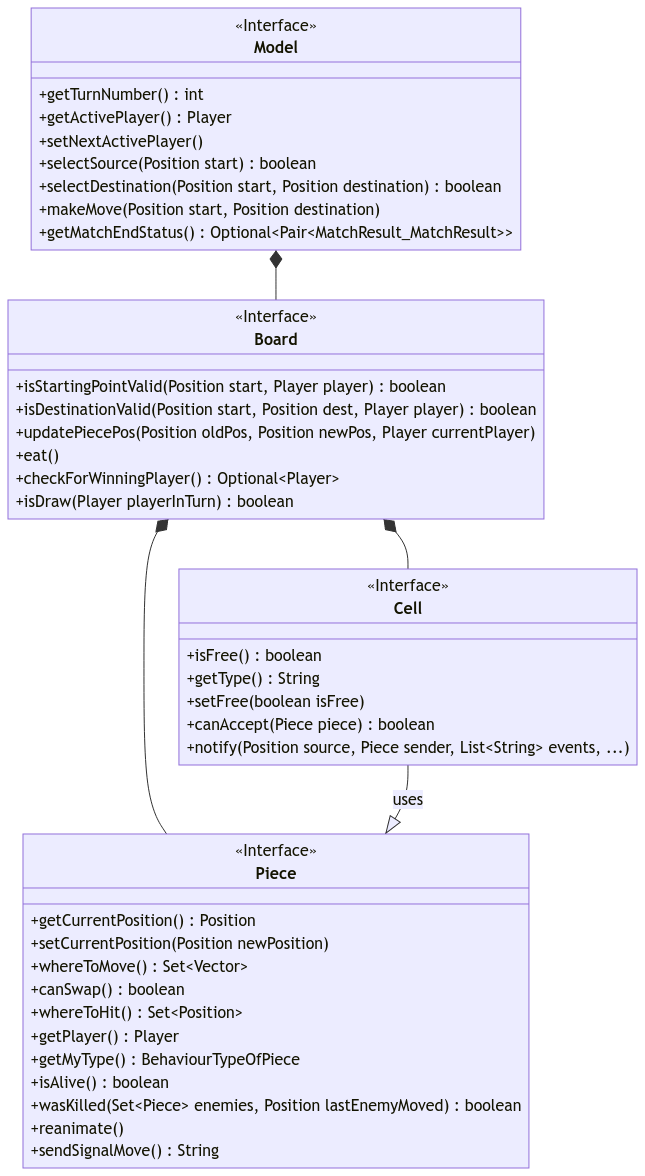
\includegraphics[width=0.8\textwidth]{images/analysis.png}
\caption{Schema UML del modello del dominio.}
\label{images:analysis}
\end{figure}

\chapter{Design}

\section{Architettura}

Come pattern architetturale, è stato scelto MVC in quanto permette di separare la logica dell'applicazione da ciò che viene mostrato all'utente, portando ad un'organizzazione interna dell'applicazione più pulita e più facilmente gestibile.

L'interfaccia \texttt{Model} racchiude la logica del dominio di gioco, isolandola da tutti gli altri componenti dell'architettura. Idealmente, il gioco potrebbe funzionare anche senza alcuna componente grafica, direttamente ricevendo input da linea di comando.

Il \texttt{Controller} si occupa del coordinamento fra Model e View, permettendo ai cambiamenti di stato della partita di essere visualizzati dall'utente. Il Controller gestisce anche alcune risorse non inerenti alla parte grafica dell'applicazione, ad esempio file di configurazione per il setup della partita e file per il salvataggio e il caricamento della leaderboard.

La \texttt{View} si occupa del rendering grafico delle varie schermate dell'applicazione. A ciascuna schermata è associata una specifica \texttt{Scene} e ciascuna di esse è legata ad un proprio \texttt{SceneController} che gestisce il comportamento della scena e la comunicazione tra la \texttt{Scene} stessa, la \texttt{View} (la quale è, in pratica, un container di \texttt{Scene}) e il \texttt{Controller}.

\section{Design dettagliato}

\subsection{Alin Stefan Bordeianu}

\subsubsection{Annullamento delle mosse}

L'utente deve avere la possibilità di annullare la propria mossa, indipendentemente dal numero di eventi che questa ha causato, e lo stato della partita a seguito di un annullamento deve tornare precisamente alla situazione precedente. Mentre per la modalità classica questo compito è relativamente facile poiché a variare sulla \texttt{Board} sono solo la collocazione delle pedine ed il loro numero in seguito a delle mangiate, nella modalità variante intervengono più elementi oltre a questi, come ad esempio le \textbf{tombe} ed il loro contenuto, gli \textbf{sliders} ed il loro orientamento, movimenti articolati come quello degli \textbf{swappers} e così via.

In ottica di estensibilità e nel rispetto del \textit{single-responsibility principle}, si rende necessario semplificare il più possibile il compito dell'unità responsabile dell'annullamento, evitando che questa sia a conoscenza dei dettagli interni di ciascuna delle entità da ripristinare ad uno stato precedente. Un altro importante problema è dato dal fatto che a ciascuna entità di cui si vuole salvare lo stato si deve poi assegnare correttamente il \textit{proprio} stato. Infatti, essendo presenti molteplici entità concettualmente simili (ad esempio, varie \texttt{Pieces} e varie \texttt{Cells}), è importante organizzare gli elementi che comporranno lo stato salvato (uno \textbf{snapshot}) in maniera da riuscire ad attribuire poi a ciascuna entità il proprio stato precedente.

Infine, l'annullamento riguarda lo stato dell'intera partita, perciò tutte le entità principali (\texttt{Match}, \texttt{Board}, \texttt{Piece} e \texttt{Cell}) devono essere ripristinate in maniera sequenziale, facendo attenzione a non creare conflitti o paradossi (del tipo, ripristinare correttamente celle e pedine sulla griglia, ma non permettere più al giocatore di turno di riprovare con una nuova mossa perché il turno non viene ripristinato).

\begin{figure}[H]
	\centering
	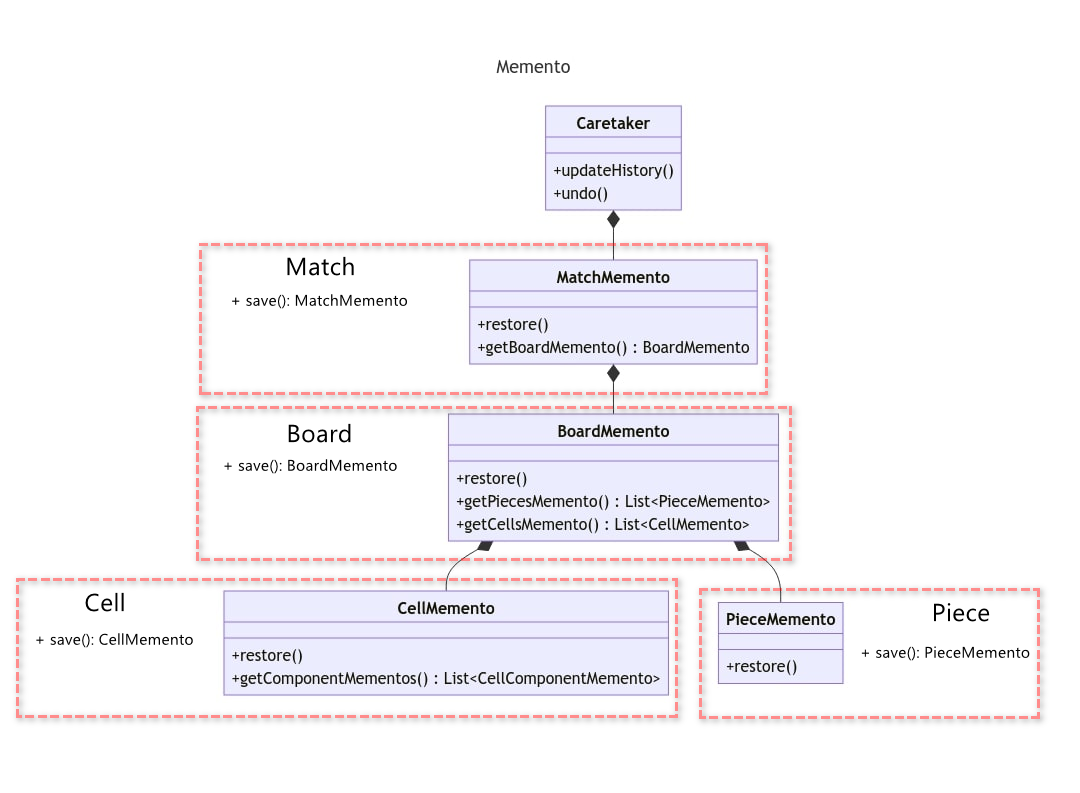
\includegraphics[width=\textwidth]{images/memento.png}
	\caption{Pattern Memento tramite Inner Classes. In figura si vede anche che ogni entità del Model ha un metodo pubblico \texttt{save()}, mentre il metodo \texttt{restore()} fa parte delle Inner Classes, che corrispondono agli snapshot delle entità. I rettangoli rossi rappresentano le Outer Classes. Per quanto concerne i \texttt{CellComponentMemento}, ci saranno più dettagli in seguito.}
	\label{images:memento}
\end{figure}

\textbf{Problema:} salvare lo stato di molteplici entità in un contenitore centrale su cui sia semplice operare, in una maniera indipendente dal contenuto delle entità e in modo tale da poter associare a ciascuna entità il proprio stato salvato. Il processo deve essere il più automatico possibile, in quanto ripristinare lo stato su ciascuna singola entità "manualmente" è estremamente brigoso a livello di chiamate di codice e può causare errori facilmente.
\\\\
\textbf{Soluzione:} si è adottato un sistema che riprende molti concetti del \textbf{pattern Memento} nella sua variante che sfrutta le Inner Classes del linguaggio Java, come visibile nella figura \ref{images:memento}. Tali Inner Classes sono pubbliche e per loro natura hanno accesso ai campi, anche privati, della Outer Class che le contiene. La variazione rispetto al pattern tuttavia consiste nel fatto che la chiamata al metodo di ripristino \texttt{restore()} non avviene sull'Originator (ossia l'entità che ha generato lo stato salvato, chiamato da qui in poi \textbf{"memento"}), ma sul memento stesso. Il vantaggio di questo approccio è che il memento, che altro non è che un'istanza di una Inner Class, ha sempre un riferimento alla Outer Class che lo ha generato. In questa maniera il Caretaker, cioè l'entità con lo scopo di mantenere lo storico dei memento, \textbf{non deve preoccuparsi di fare l'associazione fra ogni memento e l'entità che lo ha creato.}

Per quanto riguarda il ripristino delle entità nel corretto ordine, i vari memento sono stati composti fra di loro; in altre parole, a livello più basso ci sono i \texttt{CellMemento} e i \texttt{PieceMemento} che contengono, salvo eccezioni, soltanto informazioni sullo stato delle entità a cui si riferiscono; il \texttt{BoardMemento} contiene una collezione di \texttt{CellMemento} e \texttt{PieceMemento} oltre alle informazioni rilevanti sullo stato della \texttt{Board}, e infine il \texttt{MatchMemento} contiene un \texttt{BoardMemento}. Per salvare lo stato di una partita si crea un oggetto \texttt{CaretakerImpl}, il quale implementa l'interfaccia \texttt{Caretaker} e mantiene un riferimento ad una partita, e si chiama su di esso il metodo \texttt{updateHistory()}. Questo genera una catena di chiamate ai vari metodi pubblici \texttt{save()} delle entità che costituiscono il modello del dominio, e il risultato finale sarà un semplice \texttt{MatchMemento} che verrà conservato all'interno di uno Stack (inteso come la struttura dati) nel CaretakerImpl. Per l'annullamento della mossa, sarà sufficiente chiamare il metodo \texttt{undo()} del Caretaker, che causerà la chiamata ai vari metodi \texttt{restore()} dei memento.
\\\\
Questo sistema semplificato di salvataggio degli stati della partita può essere ulteriormente espanso, portando potenzialmente alla creazione di replay che siano costituiti dal semplice susseguirsi ordinato dei MatchMemento. Al momento l'applicazione consente di tornare indietro soltanto di una mossa, per due motivi:
\begin{itemize}
	\item tornare indietro di più di una mossa significherebbe annullare anche le mosse dell'avversario, cosa che nel contesto di un gioco da tavolo non considero appropriata;
	\item il Caretaker potrebbe benissimo mantenere in memoria più di uno snapshot in linea teorica, ma esiste il rischio che tutti gli oggetti memento occupino molta RAM causando ritardi dell'applicazione. \`E stata presa in considerazione l'idea di salvare ciascun oggetto memento su file invece di tenerlo in memoria, ma per mancanza di tempo questa soluzione non è stata tentata.
\end{itemize}

\subsubsection{Leaderboard}

Si vuole tenere traccia dei risultati dei giocatori, costruendo una classifica che mostri il nome di ogni giocatore che abbia voluto registrare il risultato di una partita ed il risultato ottenuto. Tale classifica, anche denominata \textbf{leaderboard}, deve essere ordinata in base al numero di vittorie ottenute; nel caso in cui ci siano dei pareggi fra giocatori, l'ordinamento avviene considerando il numero di sconfitte (chi ne ha subite di meno avrà il posto in classifica più alto). I giocatori non avranno dei profili veri e propri, ma saranno identificati semplicemente da un nickname non vuoto che inseriranno al termine di ogni partita di cui vorranno registrare il risultato. La leaderboard deve anche poter essere svuotata. La leaderboard costituisce un dato persistente, che dunque andrà salvato su file.
\\\\
Per effettuare il salvataggio su file è stata utilizzata la libreria esterna \textbf{SnakeYaml} (si veda la documentazione \href{https://bitbucket.org/snakeyaml/snakeyaml/wiki/Documentation}{qui}), in quanto le associazioni fra giocatori e punteggi erano facilmente rappresentabili da una Map e la sintassi di Yaml consentiva un facile passaggio da e su file in questo caso. Un problema riscontrato in questa fase è stato quello di trovarsi alle prese con il salvataggio di oggetti generici \texttt{Pair<X, Y>} che causavano difficoltà non indifferenti per via dei generici non reificati del linguaggio Java, ma alla fine ho optato per una soluzione più semplice che facesse uso di variabili facilmente gestibili come stringhe e interi, costruendo le Pair dinamicamente dopo la lettura di tali dati dal file.

\begin{figure}[H]
	\centering
	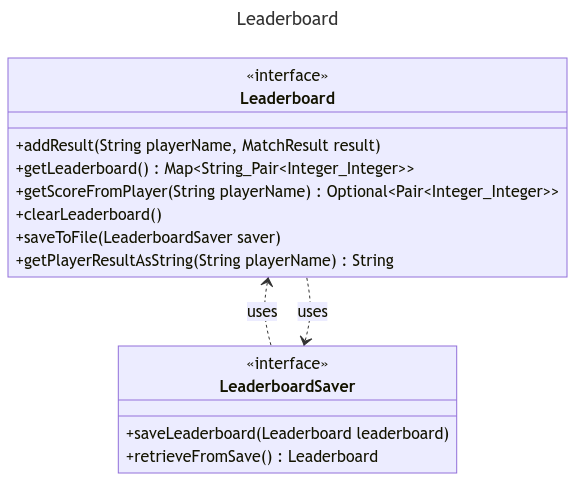
\includegraphics[width=\textwidth]{images/leaderboard.png}
	\caption{Diagramma UML che mostra i metodi delle interfacce Leaderboard e LeaderboardSaver.}
	\label{images:leaderboard}
\end{figure}

La logica del salvataggio è stata inserita nel \texttt{LeaderboardSaver} (figura \ref{images:leaderboard}), mentre la gestione della leaderboard intesa come possibilità di aggiungere risultati e mostrare una classifica ordinata è affidata alla classe \texttt{Leaderboard} (figura \ref{images:leaderboard}). Il metodo \texttt{getPlayerResultAsString(String playerName)} è presente in vista di una potenziale funzionalità di filtraggio dei risultati della classifica, ma al momento per ragioni di tempo non è stato sfruttato nella creazione dell'interfaccia grafica. La \texttt{Scene} riservata alla visualizzazione della leaderboard è la \texttt{HighScoreScene}, pilotata dal \texttt{HighScoreController}. All'utente è consentito visualizzare e svuotare la leaderboard.

\subsubsection{Tombe come CellComponents}

La Tomba è un'entità particolare della modalità variante che viene piazzata sulla griglia di gioco in corrispondenza delle coordinate a cui è morta una qualsiasi pedina. Durante la fase di analisi la \texttt{Tomb} è sempre stata considerata come una \texttt{Cell} a tutti gli effetti. Tuttavia quando si è giunti al punto di dover scrivere il codice che creasse le Tombe una volta morte le pedine, sono emersi alcuni problemi legati a questa visione della Tomba:
\begin{itemize}
	\item la Tomba non deve rimpiazzare gli eventuali effetti delle celle su cui viene generata;
	\item se una Tomba è vuota, deve poter essere rimossa tranquillamente senza il rischio di lasciare un buco nella griglia, e preferibilmente senza che entità esterne debbano memorizzare che tipo di cella era collocata a tali coordinate in precedenza;
	\item lo stato della Tomba deve poter essere salvato agevolmente per permettere al giocatore di annullare una mossa in maniera coerente con le altre entità che producono dei memento, ma anche lo stato della cella precedente all'inserimento della Tomba deve essere mantenuto, il che implica che la cella precedente non dovrebbe essere eliminata.
\end{itemize}

\begin{figure}[H]
	\centering
	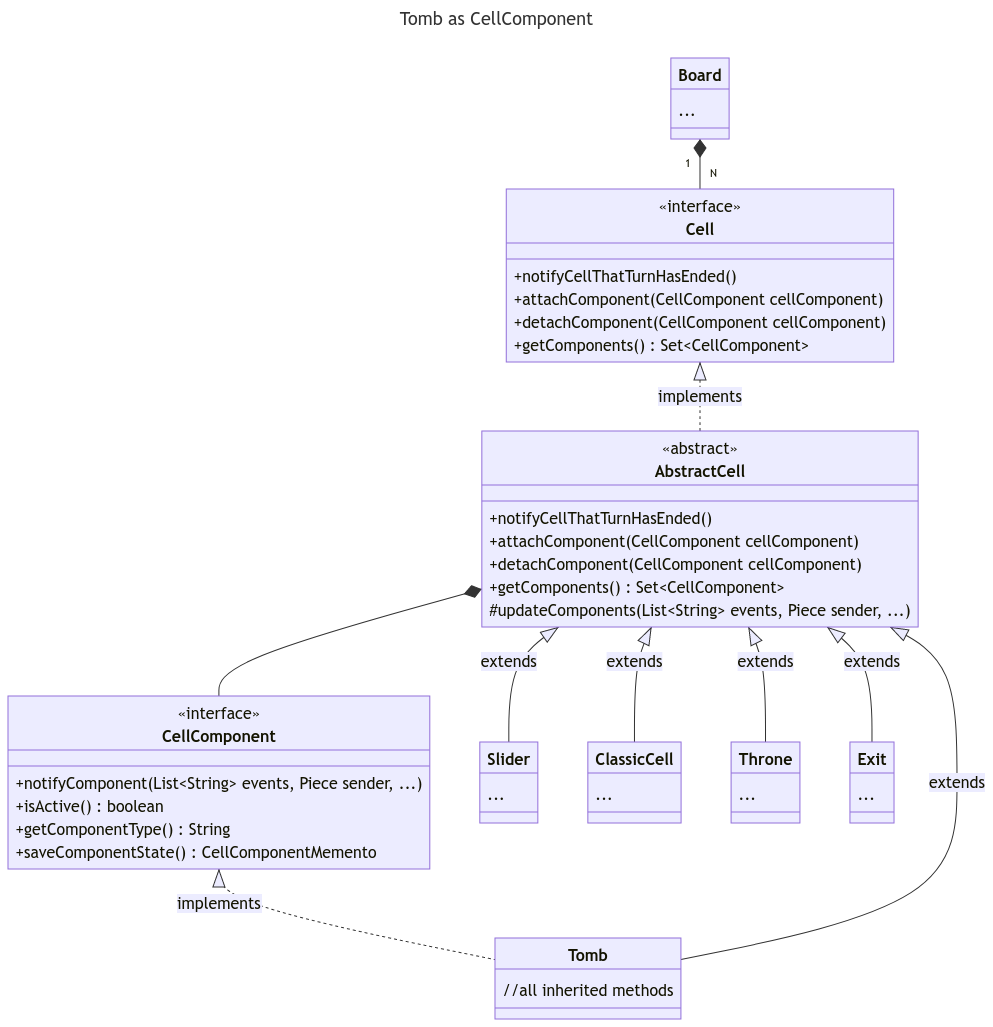
\includegraphics[width=\textwidth]{images/tomb-as-cellcomponent.png}
	\caption{\texttt{Tomb} viene ora trattata come un CellComponent, che può essere attaccato o staccato a seconda di certi eventi che la \texttt{Board} si occuperà di rendere noti alla \texttt{Cell}.}
	\label{images:tomb-as-cellcomponent}
\end{figure}

\textbf{Problema:} realizzare la \texttt{Tomb} in una maniera che catturi meglio la sua natura di caratteristica opzionale di \texttt{Cell} già esistenti, senza rimpiazzare le \texttt{Cells} già presenti alle coordinate della morte di una pedina.
\\\\
\textbf{Soluzione:} si è scelto di trattare la Tomba non più come una Cella a sé stante, ma come un componente da poter attaccare e staccare alle \texttt{Cells} normali (figura \ref{images:tomb-as-cellcomponent}). Per farlo è stato applicato il \textbf{pattern Composite}. Il \textbf{base component} è costituito dall'interfaccia \texttt{Cell}, che è il genere di entità di alto livello con cui opera la \texttt{Board}, la quale funge da \textbf{client}. I \textbf{leaf components}, ossia quelli che non hanno riferimento agli altri componenti e forniscono una implementazione base dei metodi del componente di base, sono tutte le celle ad eccezione della \texttt{Tomb}: \texttt{ClassicCell}, \texttt{Throne}, \texttt{Exit} e \texttt{Slider}. A fare da \textbf{composite} c'è la classe astratta \texttt{AbstractCell}, che implementa \texttt{Cell} e contiene la logica per attaccare, staccare e aggiornare i componenti. Infine la \texttt{Tomb} viene ora trattata come un \texttt{CellComponent}, e per piazzarne una su una qualsiasi altra casella è sufficiente che il client (la \texttt{Board}) attacchi un nuovo componente ad una \texttt{Cell} (questo avviene indirettamente tramite vari metodi che notificano eventi che potrebbero essere rilevanti o meno per le specifiche caselle). Per evitare duplicazioni di componenti, l'\texttt{AbstractCell} ha un Set di \texttt{CellComponents}. Ogni \texttt{CellComponent} ha anche un metodo \texttt{isActive()} mediante il quale può essere monitorato per capire quando è possibile staccarlo. Più in dettaglio, se la \texttt{Tomb} non contiene più alcun pezzo perché tutti sono stati resuscitati, allora la  \texttt{AbstractCell} stacca in autonomia tale componente quando viene notificata dalla \texttt{Board} che il turno è finito.
\textit{Nota: sebbene in questa sottosezione vengano nominate molte classi, soltanto i metodi che riguardano il salvataggio dei CellMemento e i CellComponents sono mia responsabilità.}

\subsection{Elena Boschetti}

\subsubsection{Match setup}

La fase di setup della partita prevede la creazione della griglia di gioco e la disposizione delle pedine su di essa; in termini di codice, ciò corrisponde alla creazione di un oggetto di tipo \texttt{Board} e all'inizializzazione delle collezioni di celle e pedine che essa conserva internamente. 

La costruzione delle due collezioni fa uso di due diversi builder: \\ \texttt{CellsCollectionBuilder} per la collezione di celle e \texttt{PiecesCollectionBuilder} per la collezione di pedine. Ogni metodo delle interfacce dei builder permette di aggiungere alle collezioni un sottoinsiemi di pedine e celle di un determinato tipo. Da notare che i builder ricevono le coordinate a cui posizionare celle e pedine dall'esterno (in quanto passate come parametri ai diversi metodi), quindi i builder operano in maniera indipendente dal modo in cui la configurazione iniziale di celle e pedine viene fornita.

La configurazione iniziale dipende dalla modalità di gioco (classica o variante). Il caricamento della configurazione per ogni modalità viene avviato mediante l'interfaccia \texttt{SettingsLoader}. Dietro tale interfaccia, si possono definire diverse possibilità per quanto riguarda il reperimento della configurazione, creando per ciascuna di esse una classe che implementi l'interfaccia. L'implementazione di \texttt{SettingsLoader} da me definita prevede il caricamento della configurazione da un file XML (uno per ogni modalità di gioco), ma sarebbe possibile definire altre classi che la ottengano in maniera differente. È una possibilità che potrebbe essere utile anche nel caso in cui si verifichino problemi: ad esempio, se il caricamento da file XML non va a buon fine per qualche motivo, si può decidere di procedere per una via alternativa, creando un nuovo tipo di loader che cerchi di reperire la configurazione in altro modo.

Per costruire le collezioni di pedine e celle secondo la configurazione, il \texttt{SettingsLoader} riceve un \texttt{CellsCollectionBuilder} e un \\ \texttt{PiecesCollectionBuilder} e interagisce con essi per creare e posizionare correttamente ogni tipologia di celle e pedine; ad esempio, il \texttt{SettingsLoader} ottiene le posizioni delle Exit Cells e successivamente chiama il metodo \texttt{addExits()} del \texttt{CellsCollectionBuilder}, passando tali posizioni. Una volta completata la costruzione delle due collezioni, esse vengono passate alla \texttt{Board} che viene istanziata, la quale viene a sua volta passata all'istanza di \texttt{Match} che viene creata.

\begin{figure}[H]
\centering
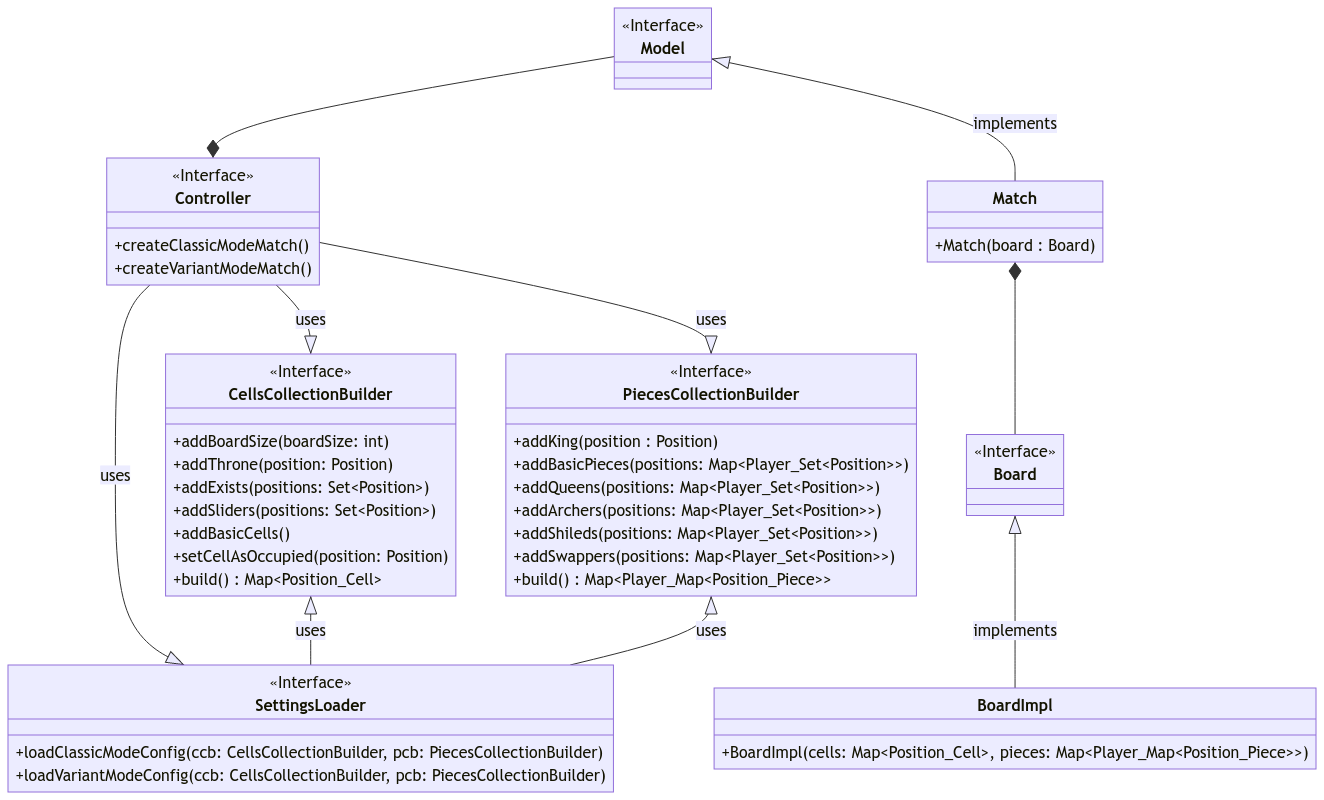
\includegraphics[width=\textwidth]{images/match-setup.png}
\caption{Schema UML che rappresenta l'interazione tra le entità coinvolte nel setup.}
\label{images:match-setup}
\end{figure}

\subsubsection{Scenes}

La view dell'applicazione, realizzata utilizzando la Java Swing API, è composta da un serie di scene.
L'implementazione della \texttt{View} prevede la creazione del container più esterno della view (un \texttt{JFrame}) e l'alternarsi delle diverse scene viene gestito impostando il frame con un opportuno layout (\texttt{CardLayout}) che consente di sostituire il container interno (un \texttt{JPanel}) che viene mostrato, il quale corrisponde alla scena.

Considerando la chiara differenza di ogni scena a livello grafico e le differenze di comportamento che ogni scena può avere (ad esempio, in risposta ad un input dell'utente), ho deciso di racchiudere il concetto di scena in un'entità a sè stante. L'interazione diretta con ogni scena avviene mediante l'interfaccia \texttt{Scene}, la quale consente di ottenere il container che costituisce la scena e di interagire con essa, ad esempio per il suo aggiornamento mediante il metodo \texttt{update()}. L'implementazione della \texttt{View} ha un riferimento alla \texttt{Scene} attualmente mostrata, il quale permette che un'interazione con la \texttt{View} abbia un effetto sulla scena corrente; ad esempio, se il controller dell'applicazione richiede l'aggiornamento della view mediante il metodo \texttt{update()} della \texttt{View}, in tale metodo viene richiamato il metodo \texttt{update()} della scena corrente.

Riflettendo sugli aspetti comuni che possono esserci tra le scene (ad esempio, la creazione del container e alcune sue impostazioni, oppure l'uso di altri parametri comuni, come il font) ho ritenuto che fosse utile definire una classe astratta (\texttt{AbstractScene}) che implementasse tali aspetti comuni tra le scene. 

Le implementazioni concrete di ogni scena estendono \texttt{AbstractScene} e definiscono tutto ciò che è inerente alla specifica scena; in particolare, ogni classe costruisce la parte grafica della scena e definisce altri eventuali metodi utili all'interazione dalla \texttt{View} alla scena. Ad esempio, qualora una scena debba avere un aggiornamento a seguito di un input dell'utente, esso può essere innescato chiamando il metodo \texttt{update()}, come detto precedentemente.

\begin{figure}[H]
\centering
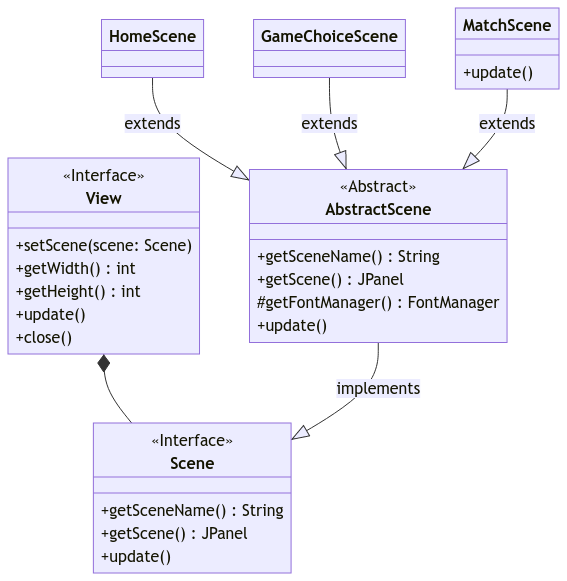
\includegraphics[width=0.75\textwidth]{images/scenes.png}
\caption{Schema UML che rappresenta il rapporto tra le entità che descrivono le scene della view. Sono mostrate solo le classi concrete che definiscono la schermata iniziale dell'applicazione (\texttt{HomeScene}), la schermata della scelta della modalità di gioco (\texttt{GameChoiceScene}) e la schermata della partita (\texttt{MatchScene}) a titolo esemplificativo.}
\label{images:scenes}
\end{figure}

In seguito a questa fase di design, mi sono occupata di implementare la scena della home del gioco (\texttt{HomeScene}), la scena della scelta della modalità di gioco (\texttt{GameChoiceScene}) e della scena che mostra il regolamento (\texttt{RulesScene}).

\subsubsection{Scene Controllers}

Nello sviluppo delle funzionalità delle scene, si è rivelato quasi sempre necessario che la scena interagisse con la \texttt{View} (che, come detto precedentemente, ha la funzione di wrapper della scena) o con il Controller dell'applicazione. Per questo motivo, ho deciso di introdurre delle entità, a cui mi riferisco con il termine "scene controllers", che regolano il comportamento della scena e che hanno il ruolo di mediatore tra \texttt{Scene}, \texttt{View} e \texttt{Controller}.

Tutte le scene hanno alcune funzionalità e necessità in comune, come il passaggio alla scena successiva o precedente e la necessità di conoscere le dimensioni della view per dimensionare i componenti interni; per questo motivo, ho deciso di raggruppare queste in un'unica interfaccia (\texttt{BasicSceneController}). Successivamente, ho notato che gli scene controllers condividevano anche parte della loro implementazione: ad esempio, contengono tutti un riferimento alla \texttt{View} e al \texttt{Controller} e ottengono dalla view le informazioni utili per il dimensionamento nello stesso modo; ho quindi deciso di realizzare una classe astratta (\texttt{AbstractSceneController}) che implementasse tali aspetti comuni.

Ogni scena ha poi le proprie specifiche funzionalità; ciò rende necessario che lo scene controller di ogni scena fornisca degli ulteriori metodi per poterle attuare, oltre a quelli stabiliti nel \texttt{BasicSceneController}. Ad esempio, Lo scene controller della home scene permette anche il passaggio alla scena che mostra gli high scores e permette di comunicare alla \texttt{View} la richiesta di chiusura dell'applicazione. Lo scene controller della scena di scelta del gioco, invece, permette la creazione della partita nella modalità scelta e permette di passare alla scena che mostra il regolamento di gioco. Ho quindi deciso che, per ogni scena, il rispettivo scene controller dovesse avere una propria interfaccia, che estendesse \texttt{BasicSceneController} (si veda la \Cref{images:scene-controllers-interfaces} in relazione agli esempi appena fatti). 

\begin{figure}[H]
\centering
\subfloat{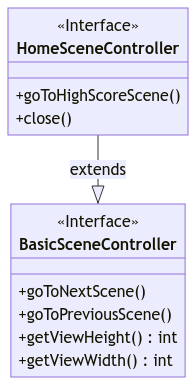
\includegraphics[width=0.3\textwidth]{images/home-scene-controller-interface.png}}
\subfloat{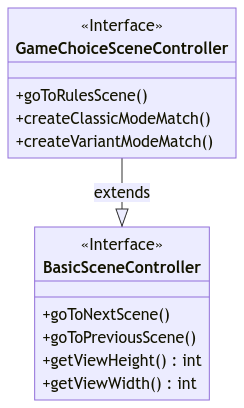
\includegraphics[width=0.3\textwidth]{images/game-choice-scene-controller-interface.png}}
\caption{Due esempi di interfaccia di due scene controllers.}
\label{images:scene-controllers-interfaces}
\end{figure}

L'implementazione di ogni scene controller deve quindi implementare la sua specifica interfaccia e estendere \texttt{AbstractSceneController}; di fatto, essa consiste solo nell'implementazione delle funzionalità specifiche della rispettiva scena.

\begin{figure}[H]
\centering
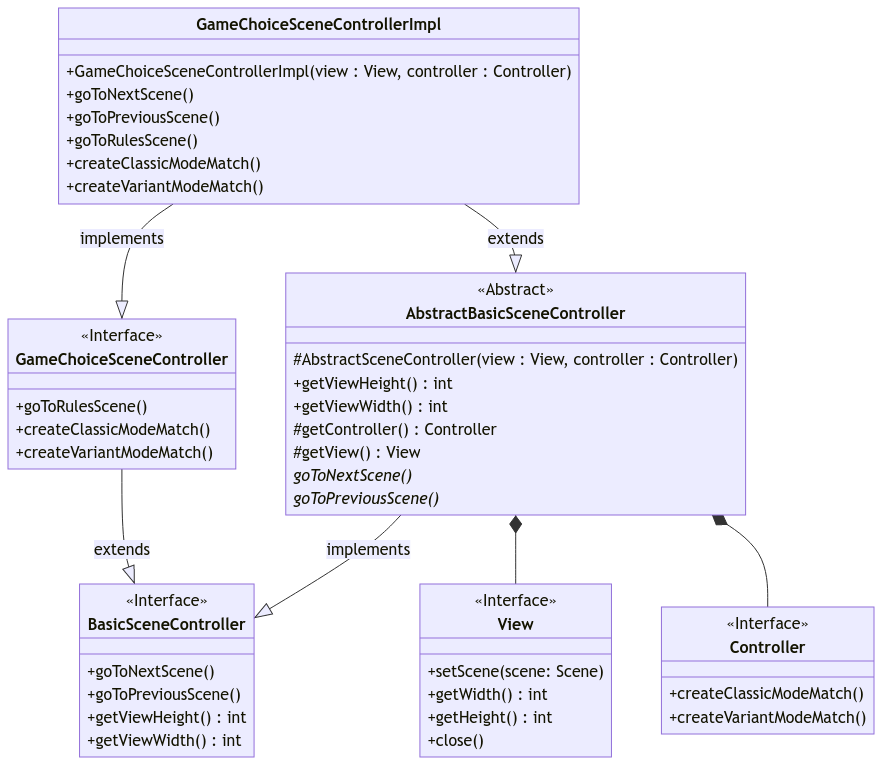
\includegraphics[width=\textwidth]{images/game-choice-scene-controller.png}
\caption{Schema UML che rappresenta il design di uno scene controller (in questo caso, lo scene controller della scena di scelta del gioco).}
\label{images:game-choice-scene-controller}
\end{figure}

In seguito a questa fase di design, mi sono occupata di implementare gli scene controller delle scene di mia competenza.

\subsection{Andrea Piermattei}
\subsubsection{Progettazione delle pedine}
I criteri principali che ho cercato di rispettare durante l'intero processo di progettazione delle pedine sono:
\begin{itemize}
\item \textbf{semplicità} e \textbf{flessibilità} nel creare sia nuovi tipi di pedine, sia istanze di pedine e nel modificare quelle già esistenti;
\item progettare classi relativamente \textbf{semplici} e \textbf{specializzate}, che possano operare il più \textbf{indipendentemente} possibile tra loro;
\item \textbf{estendibilità} del codice.
\end{itemize}

Per rispettare questi criteri sono stati usati questi tipi di \textbf{pattern}:
\begin{itemize}
\item un pattern ispirato al \textbf{pattern component} (interfacce correlate \texttt{BehaviourTypeOfPiece})
\item tre \textbf{factory methods} distinte (interfacce correlate: \texttt{FactoryHitbox}, \texttt{FactoryMoveset}, \texttt{FactoryBehaviourTypeOfPiece})
\end{itemize}

Per poter capire meglio il pattern che ho creato, vorrei spiegare brevemente in cosa consiste il pattern component.
Questo tipo di pattern è caratterizzato da un'unica \textbf{entità} che si occupa di più \textbf{domini} distinti tra loro. Ognuno di essi
ha un compito ben preciso ed è contenuto all'interno di una classe a parte, che chiameremo \textbf{component}. In questo modo \textbf{l'entità
principale} che si vuole modellare, non è altro che un \textbf{contenitore} di component a cui vengono delegati i compiti da fare. Un esempio
di pattern component è il GameObject che può possedere più componenti: GraphycsComponent, InputComponent, PhysicsController...
La scelta dell'architettura usata nell'applicazione e la natura stessa delle pedine mi hanno portato ad usare una versione \textbf{semplificata} e 
\textbf{specializzata} del pattern component. Al posto della classe estremamente generica GameObject, abbiamo una classe più specializzata, nominata \texttt{Piece} 
(l'interfaccia principale implementata da \texttt{AbstractPiece} che comunica direttamente con la \texttt{Board}), che rappresenta i \textbf{pezzi generici} che l'utente può muovere durante la partita. 
Essa contiene tutti i campi e i metodi comuni alle pedine \textbf{indipendentemente} dal loro tipo, come per esempio
la posizione corrente, la squadra di appartenenza e il numero corrente di vite.
Bisogna però specificare che quest'ultimo viene inizializzato con il numero totale di vite contenuto in \texttt{BehaviourTypeOfPiece}. L'unico componente dell'\texttt{AbstractPiece} è la
\texttt{BehaviourTypeOfPiece} (implementato da \texttt{AbstractBehaviourTypeOfPiece}), 
che contiene tutti i metodi e i campi che caratterizzano il comportamento di uno specifico tipo di pedina, quali la hitBox e la moveSet assolute 
(create prendendo come punto di riferimento la posizione (0,0)), il numero totale
di vite e i metodi abstract \texttt{.wasHit(...)}, \texttt{.generate()}, \texttt{.generateHitbox()} e \texttt{.generateMoveSet()}.
\begin{figure}[H]
\centering
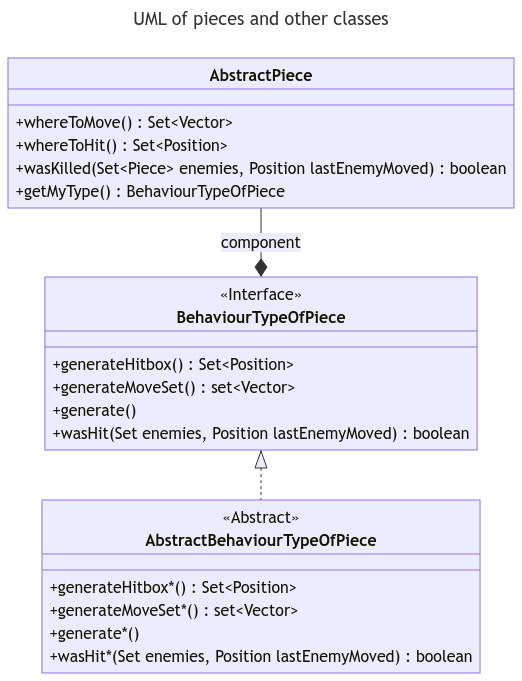
\includegraphics[width=\textwidth]{images/component-pattern.png}
\caption{Schema UML che rappresenta il design del pattern ispirato al pattern component.}
\label{images:component-pattern}
\end{figure}
Questo sistema ha alcuni vantaggi: 
\begin{itemize}
\item nel caso in cui volessi aggiungere nuove funzionalità o fare degli accorgimenti a \texttt{TypeBehaviourOfPiece}, non è detto che sia costretto a modificare il
codice già esistente della \texttt{AbstractPiece} (se non qualche piccola aggiunta);
\item semplifica la classe \texttt{AbstractPiece}.
\end{itemize}
Insieme al pattern component vengono anche usate tre \textbf{factory method} diverse:
\begin{itemize} 
\item \texttt{FactoryHitbox} (interfaccia implementata da \texttt{ImplFactoryHitbox}): crea diversi tipi di hibox assolute.
\item \texttt{FactoryMoveset} (interfaccia implementata da \texttt{ImplFactoryMoveset}): crea diversi tipi di moveset assolute.
Queste prime due factory vengono utilizzate dentro la \texttt{AbstractBehaviourTypeOfPiece}, ma possono essere usati anche da altre entità.
\item \texttt{FactoryBehaviourTypeOfPiece} (interfaccia implementata da \texttt{ImplFactoryBehaviourTypeOfPiece}): si trova all'interno della \texttt{AbstractPiece} e
crea i diversi tipi di component \texttt{BehaviourTypeOfPiece}, che verranno usati dalle classi che estendono \texttt{AbstractPiece} (cioè le \textbf{pedine effettive} che verranno usate dalla \texttt{Board}). E' qui che bisognerà 
implementare i metodi abstract della \texttt{AbstractBehaviourTypeOfPiece}.
\end{itemize}
\begin{figure}[H]
\centering
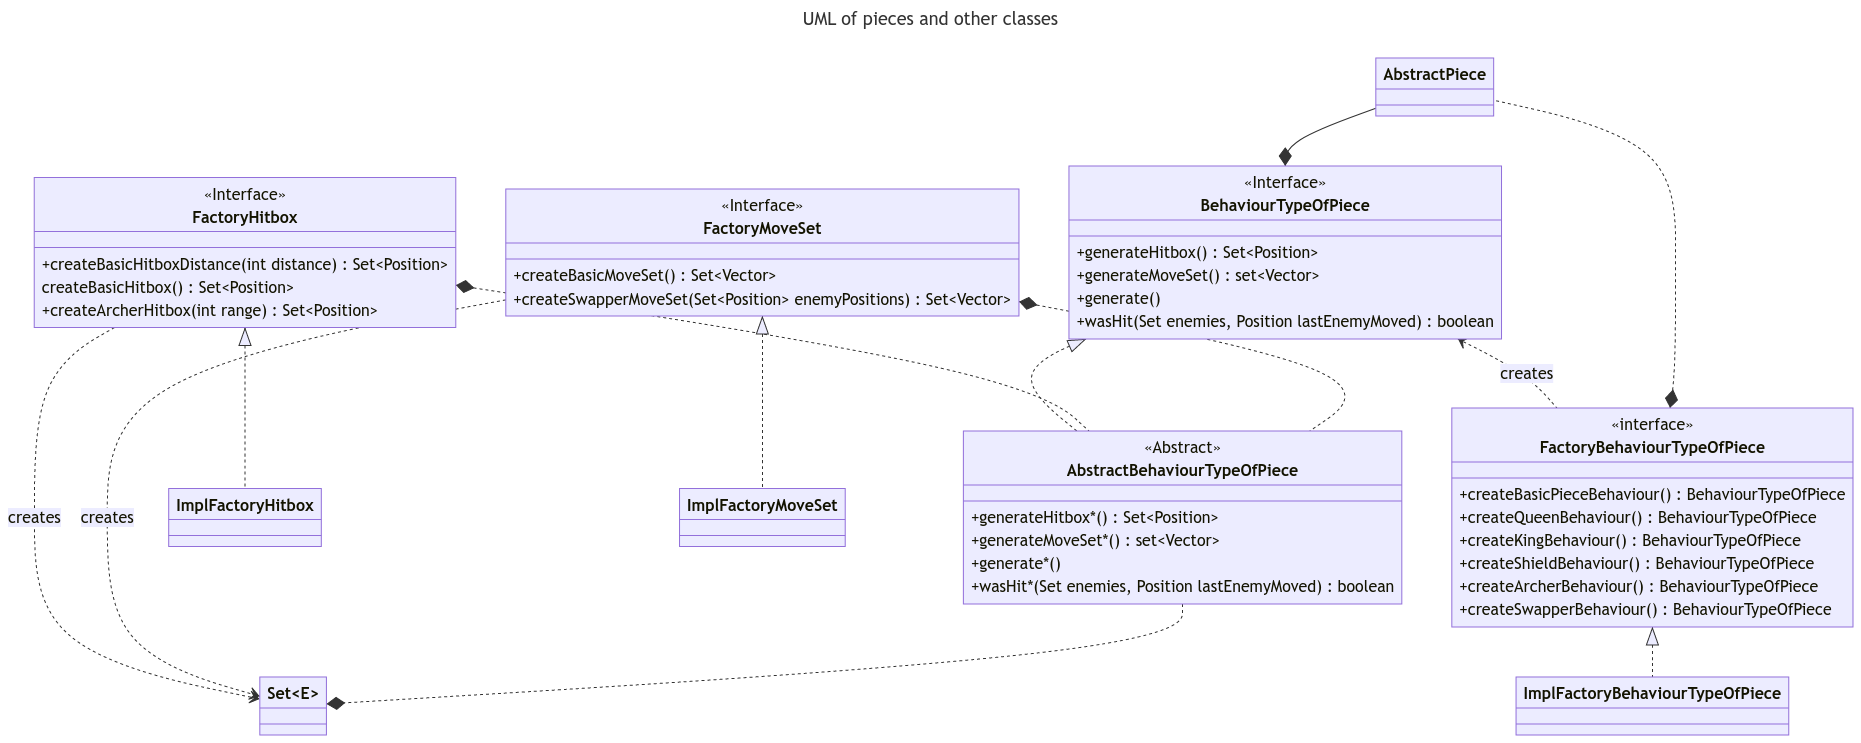
\includegraphics[width=\textwidth]{images/factory-pattern.png}
\caption{Schema UML che rappresenta i tre factory method.}
\label{images:factory-pattern}
\end{figure}
Questo sistema ci permette di semplificare il codice da scrivere sia nella \texttt{TypeBehaviourOfPiece} per la scelta delle \texttt{hitbox} e \texttt{moveset}, sia nelle implementazioni delle pedine che estendono \texttt{AbstractPiece}
per sceglire la \texttt{BehaviourTypeOfPiece}; basta infatti chiamare all'interno della classe il metodo desiderato della \textbf{factory} in questione che farà tutto ciò che serve.
L'utilizzo di questi due pattern ci permette di creare implementazioni di pedine molto piccole e facili da usare da entità esterne come la \texttt{Board}; il loro costruttore ha bisogno di sapere solo qual è la \textbf{posizione iniziale} e il \textbf{player} a cui appartiene.

\subsubsection{Meccanica della mangiata delle pedine}

La meccanica della mangiata all'interno delle pedine è rappresentata dai due metodi \texttt{.wasKilled(...)} di \texttt{Piece} e \texttt{.wasHit(...)} di \texttt{BehaviourTypeOfPiece}, i quali vengono chiamati
solo quando una pedina, che denomineremo \textbf{"vittima"}, viene \textbf{"minacciata"} da una o più pedine nemiche. Questo corrisponde a dire che la pedina
\textbf{"vittima"} si trova in corrispondenza di una o più \textbf{hitbox} nemiche. Non è detto che una pedina minacciata venga ogni volta mangiata, infatti le \textbf{condizioni 
di morte} di una pedina vengono determinate da \texttt{.wasHit(...)} a partire dai dati forniti direttamente dalla \texttt{Board} (una collezione di posizioni nemiche e l'ultima pedina nemica mossa).
La \texttt{.wasKilled(...)} si limita ad interrogare la \texttt{.wasHit(...)}.

Questo intero sistema ha dei grandi vantaggi:
\begin{itemize} 
\item rende la \texttt{Board} più semplice, visto che non si deve preoccupare di tutte le possibili combinazioni di mangiata di una pedina, ma basta che vada ad interrogare
la pedina vittima stessa;
\item possiamo creare qualsiasi tipo di \textbf{hitbox} e \textbf{condizione di morte} (cioè il contenuto di \texttt{.wasHit(...)})senza dover modificare la \texttt{Board} o la \texttt{Piece}.
\end{itemize}

\subsubsection{Altre scelte di design degne di nota}
\begin{itemize}
\item \texttt{whereToMove(...)} e \texttt{whereToHit(...)}: sono due metodi che prendono rispettivamente la moveset e la hitbox assolute contenute nel component \texttt{TypeBehaviourOfPiece} e le adattano alla posizione corrente della pedina. In questo modo evitiamo di creare questi due dati dal nulla ogni volta che viene interrogata la pedina, ma partiamo da uno 'stampo' per generare l'ouput finale.
\item \texttt{getTypeBehaviour()}: restituisce \texttt{BehaviourTypeOfPiece}, permettendoci di accedere a tutti i suoi metodi. In questo modo possiamo limitare possibili modifiche alla \texttt{AbstractPiece}, nel caso si volessero aggiungere nuove funzionalità specifiche al tipo di pedina che si vuole implementare.
\end{itemize}
\subsubsection{MatchPanel}

Questa interfaccia (implementata da \texttt{MatchPanelImpl}) estende JPanel e ha due compiti: uno di mostrare ai giocatori la \textbf{situazione attuale} del tabellone e l'altro di ricevere più \textbf{input} dall'utente. Questo JPanel è organizzato in quattro \textbf{livelli} (JPanel) ben distinti (usando un \texttt{OverlayLayout}), ognuno contenente una griglia 11x11.
\begin{itemize}
\item il primo livello contiene i \textbf{bottoni} (con il relativo \texttt{actionListener}) usati dal giocatore di turno per selezionare le pedine della sua squadra e decidere dove spostarle;
\item il secondo livello contiene le immagini delle \textbf{pedine} ancora vive;
\item il terzo livello contiene le immagine delle \textbf{celle speciali} attualmente attive;
\item il quarto rappresenta il \textbf{tavolo da gioco} e contiene le \textbf{celle di base}.
\end{itemize}
Tutti gli elementi di questi livelli sono contenuti anche dentro quattro Map distinte (\texttt{mapButtons}, \texttt{mapPieces}, \texttt{mapSpecialCells}, \texttt{mapBoard}) per
renderli più facilmente reperibili.
Il \texttt{MatchPanel} fornisce alla \texttt{MatchScene} tutti i metodi necessari per fare l'update del tavolo da gioco, 
ripulendo prima di tutto i livelli che contengono JLabel (attraverso il metodo \texttt{.removeAllIconsOnLayer(...)})
per poi ridisegnare le pedine e le celle che gli servono (attraverso i metodi \texttt{.drawAllSpecialCells(...)} e \texttt{.drawBackgroundCells(...)}). 
Per fare questo ha bisogno di reperire le immagini di pedine e celle attraverso 
i metodi dell'interfaccia LoaderImages all'interno del costruttore di MatchScene. 

\texttt{ImageInfo} è una interfaccia utilizzata per rappresentare le caratteristiche fondamentali delle immagini e di conseguenza degli oggetti 
che rappresentano. Essa è implementata dalla classe \texttt{CellImageInfo} e dalla classe \texttt{PieceImageInfo}.
\begin{figure}[H]
\centering
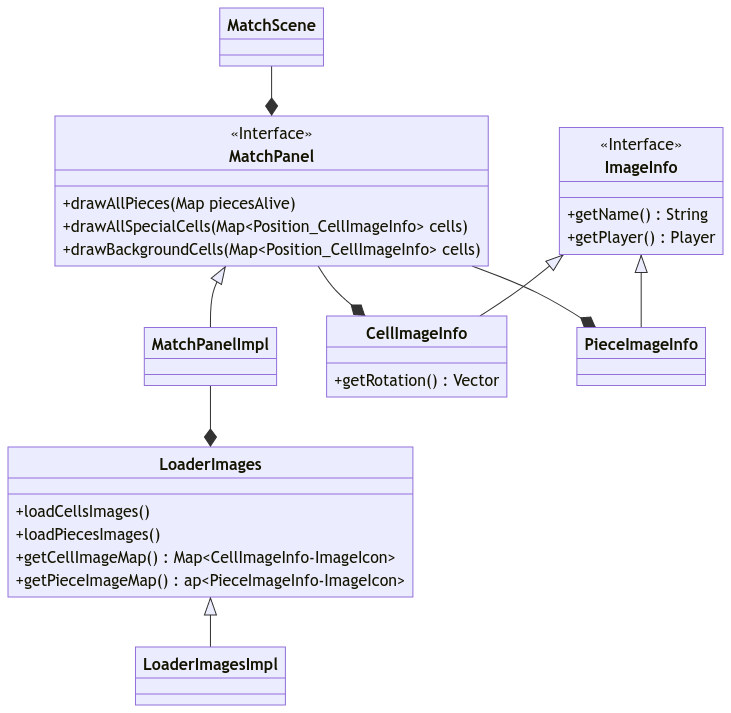
\includegraphics[width=\textwidth]{images/match-panel.png}
\caption{Schema UML che rappresenta la MatchPanel e le sue classi correlate.}
\label{images:match-panel}
\end{figure}
\subsection{Margherita Raponi}

\subsubsection{Board e Eaten}

Per modellare la logica di gioco ho identificato due momenti principali all’interno di ogni turno e ho deciso di affidarli a due oggetti distinti \texttt{Board}  e \texttt{Eaten} seguendo il \textbf{pattern Strategy}. Essendo la mangiata di uno o più pezzi un evento che al suo interno richiede di svolgere diversi controlli, ho preferito separarlo dal resto della logica di gioco implementandolo a parte in \texttt{Eaten}. Per questo motivo e in ottica di estendibilità ho scelto di sfruttare il pattern sopra citato.
All’interfaccia \texttt{Board} è affidata la logica di selezione della pedina, la logica dei controlli inerenti movimento e spostamento di quest’ultima e la logica dei controlli riguardanti lo stato della partita come la patta e la vittoria. Il setup della griglia di gioco viene passato come parametro alla \texttt{Board} attraverso due mappe: una rappresenta la disposizione delle celle sul tabellone di gioco, la seconda la disposizione delle pedine di entrambi i giocatori. Le mappe vengono passate ad inizio partita dalla classe \texttt{Match}.
La \texttt{Board} si occupa di aggiornare le due mappe in base alle azioni svolte dai giocatori. Inoltre durante ogni turno comunica con l'interfaccia \texttt{Piece}, per avere informazioni legate ai pezzi e per settarne la posizione e con l'interfaccia \texttt{Cell} per settare e avere informazioni riguardanti le celle e per notificare loro lo spostamento della pedina. In aggiunta attraverso il metodo \texttt{notifyTurnHasEnded(...)} la \texttt{Board} notifica la fine di ogni turno ad una particolare tipologia di cella detta \texttt{Slider}.
L'interfaccia \texttt{Eaten}, invece, presenta i controlli necessari per capire se un pezzo mosso ha effettuato una mangiata. Viene utilizzata dalla classe \texttt{BoardImpl} (che implementa \texttt{Board}) nel suo metodo \texttt{eat()} in cui avviene la chiamata sequenziale dei diversi metodi di \texttt{Eaten}  i quali, a loro volta, sfruttano alcuni metodi messi a disposizione da \texttt{Piece}. La \texttt{Board} stessa passa ai metodi di \texttt{Eaten} i parametri necessari per la verifica della magiata.
La scelta di isolare i controlli legati alla mangiata in una classe a parte offre la possibilità di implementare nuovi o più tipi di mangiata in eventuali future versioni del gioco.

\begin{figure}[H]
\centering
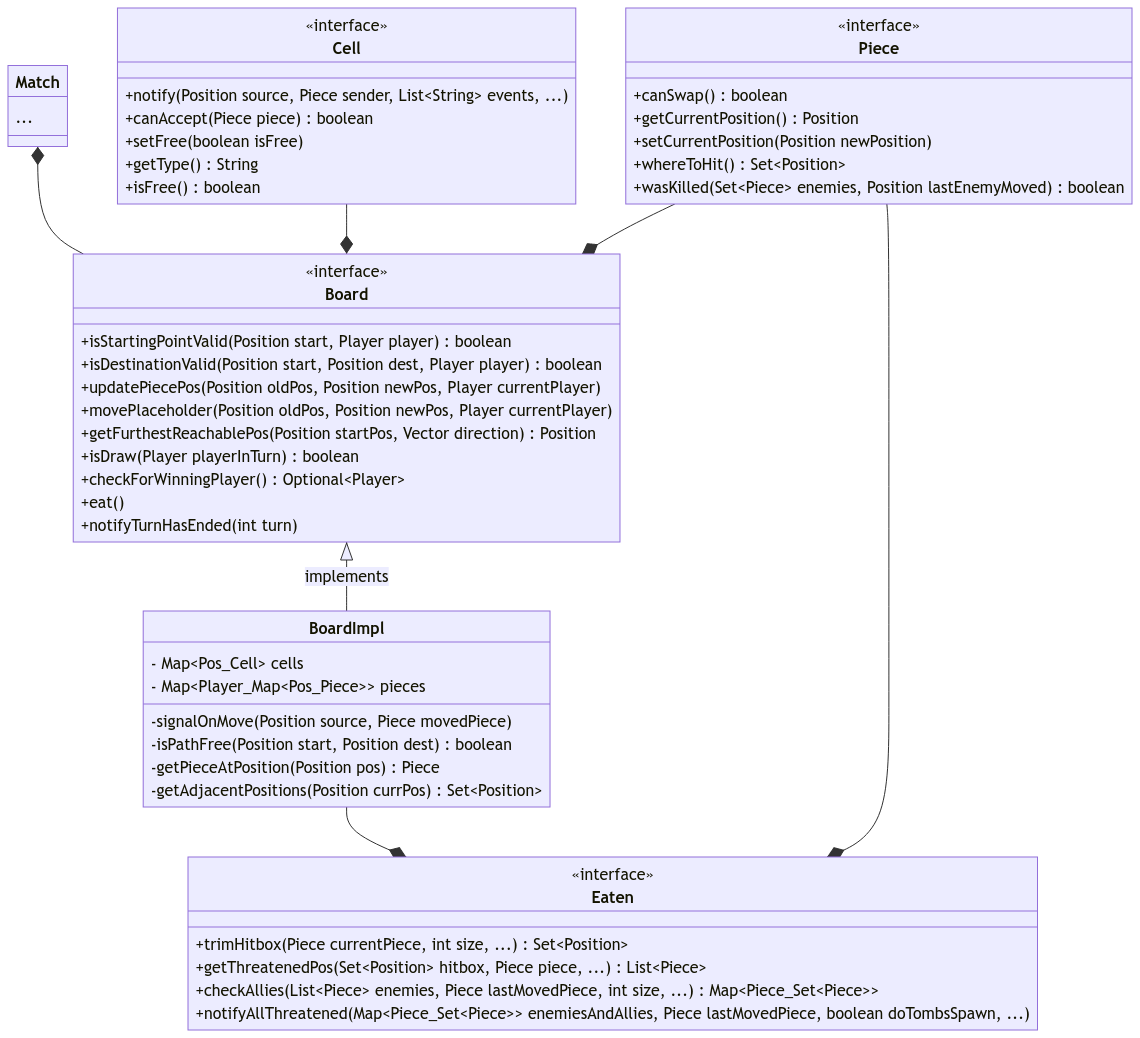
\includegraphics[width=\textwidth]{images/board-and-eaten.png}
\caption{Schema UML che rappresenta il design di Board e Eaten e delle entità a loro legate.}
\label{images:board-and-eaten}
\end{figure}

\subsubsection{Cell}

Una delle entità principali oltre alla \texttt{Board} sono le celle che compongono la griglia di gioco. 
L'interfaccia \texttt{Cell} modella le varie celle e presenta metodi che permettono di interrogarle e di settarle, ampiamente sfruttati dalla  \texttt{Board}.

\begin{figure}[H]
\centering
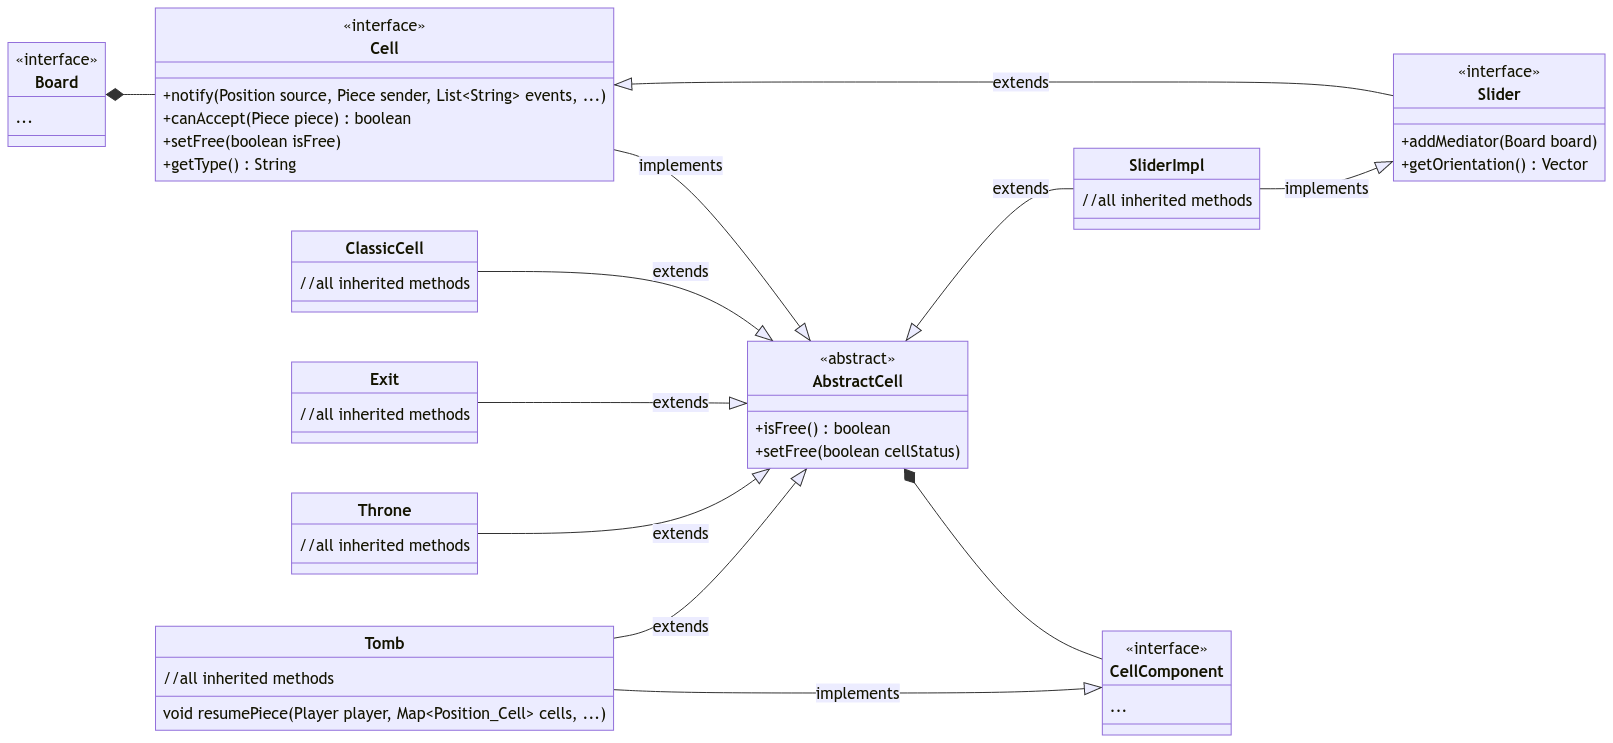
\includegraphics[width=\textwidth]{images/cells.png}
\caption{Schema UML che rappresenta il design delle celle e delle entità a loro collegate.}
\label{images:cells}
\end{figure}


\textbf{Problema:} la griglia di gioco sia della versione classica che della variante è composta da diverse tipologie di celle ognuna con un comportamento differente, in particolare nella variante è presente anche un \texttt{CellComponent} chiamato \texttt{Tomb}. Questi oggetti per quanto diversi sono caratterizzati da alcuni comportamenti comuni.
\\\\
\textbf{Soluzione:} per evitare duplicazione e ridondanza ho scelto di creare una classe astratta \texttt{AbstractCell} che implementa l’interfaccia \texttt{Cell}. \texttt{AbstractCell} implementa i metodi \texttt{setFree()} e \texttt{isFree()} comuni a tutte le celle e a \texttt{Tomb}. Ognuna delle classi che modella i diversi tipi di cella (\texttt{ClassicCell}, \texttt{Exit}, \texttt{SliderImpl}, \texttt{Throne}) e \texttt{Tomb} estende questa classe astratta aggiungendo poi i metodi necessari per completare il comportamento di quel determinato oggetto. 

\subsubsection{Slider}

Lo \texttt{Slider} è una \texttt{Cell} che presenta un effetto speciale, ovvero quando una pedina ci finisce sopra se attivo sposta la pedina nella posizione più lontana raggiungibile da quest’ultima lungo una direzione decisa dallo \texttt{Slider} stesso.

\begin{figure}[H]
\centering

\includegraphics[width=\textwidth]{images/slider.png}
\caption{Schema UML che rappresenta il design di uno Slider.}
\label{images:Slider}
\end{figure}

\textbf{Problema:}
\begin{enumerate}
\item a differenza delle altre celle lo \texttt{Slider} ha bisogno di conoscere il numero del turno e deve poter disattivarsi una volta usato poiché non si può sfruttare più volte all’interno dello stesso turno. Una volta concluso il turno deve poi riattivarsi.
\item per poter spostare il pezzo finito su esso, questa particolare cella, ha bisogno di comunicare con la \texttt{Board} per sapere in che posizione mandare il pezzo e aggiornare le due mappe che identificano le celle e le pedine del gioco.
\end{enumerate}
\textbf{Soluzione:} 
\begin{enumerate}
\item in ottica di estendibilità ho pensato che la necessità di essere aggiornati sul turno di gioco e di avere uno o più campi che devono essere resettati alla fine di ogni turno può essere una necessità anche di altre tipologie di celle che potrebbero essere implementate in futuro. Per questo motivo ho creato due interfacce \texttt{Resettable} e \texttt{TimedEntity}, la prima con un metodo per resettare i campi e la seconda con un metodo che informa sul numero del turno appena terminato. L'interfaccia Slider estende oltre a \texttt{Cell}, sia \texttt{Resettable} che \texttt{TimedEntity}.
\item ho risolto questo problema grazie al  \textbf{pattern Mediator} implementando l’interfaccia \texttt{SliderMediator} che permette a \texttt{Board} e \texttt{Slider} di comunicare, in particolare \texttt{Slider} potrà sfruttare i metodi
\texttt{getFurthestReachablePos(...)} e \texttt{movePlaceholder(...)} di \texttt{SliderMediator} per effettuare i controlli necessari per spostare il pezzo. Anche dal punto di vista dell’estendibilità l’utizzo di questo pattern può far comodo poichè evita che gli oggetti siano direttamente collegati fra loro evitando dipendenze difficili da modificare in vista di future versioni del gioco.
\end{enumerate}

\subsubsection{Caricamento delle immagini di gioco}

\begin{figure}[H]
\centering
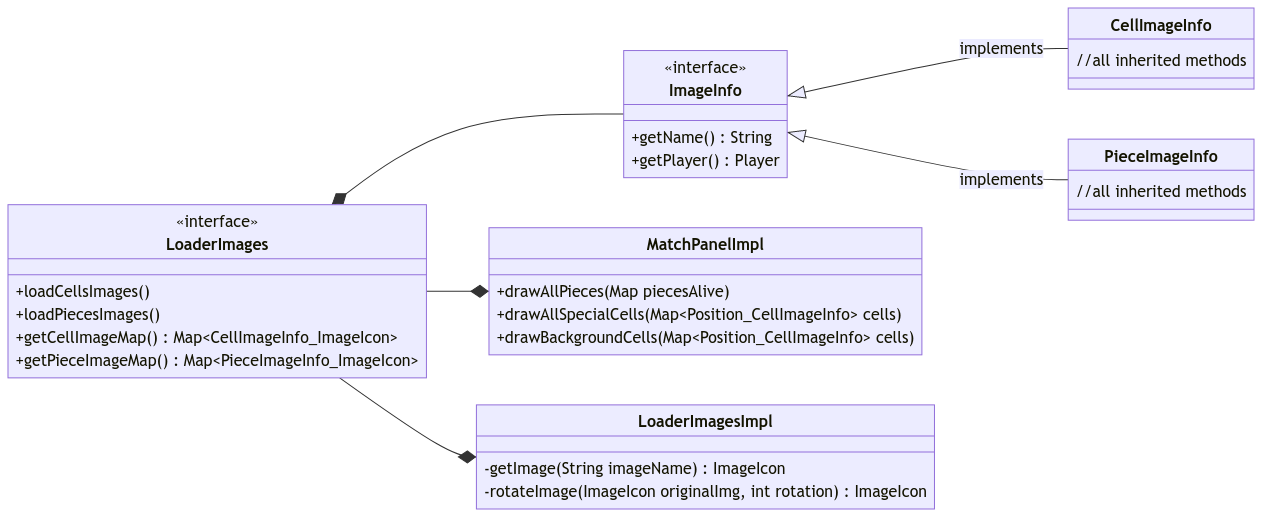
\includegraphics[width=\textwidth]{images/loader-images.png}
\caption{Schema UML che rappresenta il design dell'interfaccia \texttt{LoaderImages}.}
\label{images:loader-images}
\end{figure}

\textbf{Problema:} il gioco presenta circa una ventina di immagini per rappresentare tutte le celle e le pedine. Il caricamento di immagini risulta essere però un processo oneroso che richiede tempo, perciò non è conveniente che queste vengano caricate ogni volta all'inizio di ogni turno. 
\\\\
\textbf{Soluzione:}  l'interfaccia \texttt{LoaderImages} carica tutte le immagini necessarie al gioco all’interno di due mappe, una avrà le immagini delle pedine l’altra delle celle. All’interno di queste mappe ad ogni immagine è associato un oggetto di tipo \texttt{CellImageInfo} o \texttt{PieceImageInfo} che rispettivamente danno informazioni riguardanti il tipo cella e il tipo di pedina dell’immagine corrispondente.
Queste due mappe verranno poi sfruttate, durante tutto il corso della partita, dalla classe \texttt{MatchPanelImpl} per poter disegnare le varie entità in gioco. Questo approccio permette di caricare le immagini una sola volta all'inizio della partita e poi usufruirne  senza caricarle nuovamente. 



\chapter{Sviluppo}


\section{Testing automatizzato}


\section{Metodologia di lavoro}

\subsection{Alin Stefan Bordeianu}
In autonomia mi sono occupato di:
\begin{itemize}
	\item creazione delle classi \texttt{Position}, \texttt{Vector} e \texttt{VectorImpl} (package taflgames.common.api e taflgames.common.code), che costituiscono il principale mezzo di comunicazione di tutti gli elementi dell'architettura;
	
	\item creazione del \texttt{Caretaker}, del sistema di registrazione degli stati della partita mediante il pattern Memento, scrittura delle InnerClass che implementano le varie interfacce Memento nel caso delle \texttt{Cells} e della \texttt{Board} (package taflgames.model.memento.api e taflgames.model.memento.code);
	
	\item creazione della \texttt{Leaderboard}, del \texttt{LeaderboardSaver} e della relativa \texttt{Scene}: \texttt{HighScoreScene} e il proprio \texttt{HighScoreController};
	
	\item la creazione di un \texttt{CellImageMapper} e di un \texttt{PieceImageMapper} che potessero associare a ciascuna pedina e cella uno stato (rispettivamente \texttt{CellState} e \texttt{PieceState}) utilizzabile poi nella View (package taflgames.controller.entitystate e taflgames.controller.mapper);
	
	\item un \texttt{FontManager} e un \texttt{Limiter} (un oggetto che limitasse il numero di caratteri inseribili in dei JTextFields utilizzati per la registrazione dei risultati degli utenti);
	
	\item creazione della scena \texttt{UserRegistrationScene} e relativo \texttt{UserRegistrationController}.
	
	\item creazione della scena \texttt{GameOverScene} e relativo \texttt{GameOverController}.
\end{itemize}
In collaborazione ho lavorato:

\begin{itemize}
	
	\item con Elena Boschetti:
	
	\begin{itemize}
		
		\item sulla pianificazione di strategie per risolvere alcuni problemi fondamentali dell'applicazione, in particolare le dipendenze che le entità Tomb, Queen e Slider creavano fra i vari elementi del dominio;
		
		\item sulla realizzazione di un sistema indipendente dal sistema operativo per caricare il file leaderboard.yaml, in cui vengono salvati i risultati della Leaderboard;
		
		\item sul Controller dell'applicazione;
		
		\item sul MatchMemento, concordando sull'interfaccia da esporre al Caretaker;
				
	\end{itemize}

	\item con Andrea Piermattei:
	
	\begin{itemize}
		
		\item sulla realizzazione del PieceMemento, concordando sull'interfaccia da esporre al Caretaker;
		
		\item solo a livello di pianificazione, sul come strutturare il MatchPanel;
		
	\end{itemize}

	\item con Margherita Raponi:
	
	\begin{itemize}
		
		\item sulla creazione della Tomba mediata dalla Board, e sul sistema che l'ha resa un CellComponent;
		
		\item sul debugging della Board e dell'Eaten;
		
		\item sulla condizione di patta;
		
		\item sui test delle varie Celle e comportamenti della Board.
		
	\end{itemize}

\end{itemize}

\subsection{Andrea Piermattei}
\begin{itemize}
\item realizzazione dell'implementazione del PieceMemento (ideato da Alin)
\item progettazione e realizzazione della parte di model riguardante le pedine:
\begin{itemize}
\item FactoryHitbox e ImplFactoryHitbox
\item FactoryMoveSet e ImplFactoryMoveSet
\item BehaviourTypeOfPiece e AbstractBehaviourTypeOfPiece
\item Piece e AbstractPiece
\item Archer
\item Queen
\item King
\item Swapper
\item Shield
\item BasicPiece
\item FactoryBehaviourTypeOfPiece e ImplFactoryBehaviourTypeOfPiece
\end{itemize}
\item progettazione e realizzazione, in collaborazione con Margherita, del MatchPanel
\item creazione dell'interfaccia ImageInfo e PieceImageInfo
\item realizzazione del MatchScene in collaborazione con Margherita
\item realizzazione degli assets .png delle pedine, delle celle e l'icona
\end{itemize}

\subsection{Margherita Raponi}
In autonomia mi sono occupata di:
\begin{itemize}
	\item implementazione dell'interfacce \texttt{Board} e \texttt{Eaten}, nello specifico delle classi \texttt{BoardImpl} e \texttt{EatenImpl} che costuituiscono la logica del gioco (package taflgames.model.board.api e taflgames.model.board.code).
	\item implementazione dell'interfaccia \texttt{Cell} e delle varie classi per la creazione delle diverse tipologia di cella (package taflgames.model.cell.api e package taflgames.model.cell.code).
	\item creazione delle classi \texttt{LoaderImages} e \texttt{LoaderImagesImpl} (package taflgames.view.imagesloader).
\end{itemize}
In collaborazione ho lavorato:

\begin{itemize}
	\item con  Alin Stefan Bordeianu:
		\begin{itemize}
			\item sulla creazione della Tomba;
			\item sul debugging della \texttt{Board} e dell'\texttt{Eaten};
			\item sull'analisi delle condizioni di patta;
			\item sui test delle varie Celle e comportamenti della \texttt{Board}.
		\end{itemize}
	\item con Elena Boschetti:
		\begin{itemize}
			\item per il debugging della \texttt{Board} durante la fase di testing del \texttt{Match} e della \texttt{Board}.
		\end{itemize}
	\item con Andrea Piermattei:
		\begin{itemize}
			\item sulla realizzazione della classe \texttt{MatchPanelImpl}, implementando i metodi per disegnare le celle e implementando il comportamento dei bottoni del Panel.
			\item sulla realizzazione della classe \texttt{MatchScene}.
		\end{itemize}
\end{itemize}

\section{Note di sviluppo}

\subsection{Alin Stefan Bordeianu}

\subsubsection{Uso di Lambda expressions}
(costruttore del TombMementoImpl, metodo getLeaderboard in LeaderboardImpl)

\subsubsection{Uso di Stream}
(TestLeaderboard, tutti i memento con le varie collezioni, vari metodi restore e save)

\subsubsection{Uso di Optional}
(LeaderboardImpl in getScoreFromPlayer())

\subsubsection{Uso della libreria esterna SnakeYaml}
(LeaderboardSaverImpl)

\subsubsection{Uso della libreria SLF4J}
(LeaderboardSaverImpl)

\subsubsection{Link a parti di codice esterne e link alle risorse utilizzate:}

\begin{itemize}
	
	\item Codice della classe Pair presa dal docente: \url{https://bitbucket.org/mviroli/oop2022-esami/src/master/a01a/e1/Pair.java}
	\item Font "Latin Runes v2.0": \url{ https://www.fontget.com/font/latin-runes/}
	\item Immagine di una plancia di legno da mettere sotto alle labels della GUI: \href{https://get.pxhere.com/photo/background-tree-wood-boards-texture-wooden-background-old-brown-wood-texture-gray-wood-old-tree-old-fence-the-texture-of-the-wood-rustik-rustic-rural-wood-background-old-boards-fence-1370487.jpg}{pxhere.com}
	
\end{itemize}

\subsection{Elena Boschetti}

\subsubsection{Parsing di file XML utilizzando le funzionalità fornite dal package \texttt{javax.xml.parsers} del JDK}
Permalink: [utilizzo in SettingsLoaderImpl.java]

\subsubsection{Uso di \texttt{LoopingIterator} dalla libreria Apache Commons Collections}
Permalink: [utilizzo in Match.java]

\subsubsection{Utilizzo della libreria SLF4J}
Utilizzata in più punti. Permalinks:
\begin{itemize}
	\item utilizzo in ControllerImpl.java
	\item utilizzo in TestBoardSetup.java
	\item utilizzo in TestMatch.java
\end{itemize}

\subsubsection{Uso di \texttt{Stream} e lambda expressions}
Permalink: [utilizzo in TestBoardSetup.java]

\subsubsection{Uso di reflection}
Utilizzata in più punti nel test del setup della partita.
Permalink: [un utilizzo in TestBoardSetup.java]

\subsubsection{Scrittura di metodo generico}
Permalink: [utilizzo in TestBoardSetup.java]

\subsubsection{Uso di \texttt{Optional}}
Permalink: [utilizzo in Match.java e/o TestMatch.java]

\subsubsection{Uso di \texttt{javax.swing.text.html.HTMLEditorKit} per il rendering di file HTML}
Permalink: [uso in RulesScene.java]

\subsection{Andrea Piermattei}
\subsubsection{Uso delle lambda expressions}
Permalink:[AbstractPiece.java, ImplFactoryTypeOfPiece.java, ImplfactoryMoveset.java,MatchPanelImpl.java]

\subsubsection{Uso di \texttt{Stream}}
Permalink:[AbstractPiece.java, ImplFactoryTypeOfPiece.java, ImplfactoryMoveset.java,MatchPanelImpl.java]

\subsubsection{Uso di \texttt{Optional}}
Permalink:[MatchPanelImpl.java]

\subsection{Margherita Raponi}

\subsubsection{Uso di Stream}
Usati in vari punti. Un esempio è \url{https://github.com/Martinetto33/OOP22-tafl-games/blob/b3906dae75f2fe3908410cf72c30a889f55919ed/src/main/java/taflgames/model/board/code/BoardImpl.java#L344-L348}

\subsubsection{Uso di Lambda expressions}
Usate in vari punti. Un esempio è \url{https://github.com/Martinetto33/OOP22-tafl-games/blob/b3906dae75f2fe3908410cf72c30a889f55919ed/src/main/java/taflgames/model/board/code/EatenImpl.java#L110-L111}

\subsubsection{Uso di Optional}
Permalink: \url{https://github.com/Martinetto33/OOP22-tafl-games/blob/b3906dae75f2fe3908410cf72c30a889f55919ed/src/main/java/taflgames/model/board/code/BoardImpl.java#L374-L392}


\chapter{Commenti finali}


\section{Autovalutazione e lavori futuri}

\subsection{Alin Stefan Bordeianu}
Ho avuto l'occasione di confrontarmi con problemi non banali e ho allenato le mie capacità di trovarvi soluzioni, collaborando all'interno di un team. Grazie al tempo speso seguendo le lezioni e facendo prove per conto mio, sono stato capace di sfruttare meccanismi avanzati del linguaggio Java come gli Stream e le Lambda che mi hanno permesso di scrivere più agevolmente del codice che fosse di qualità e anche facilmente testabile.

Penso di aver fatto un buon lavoro anche per quello che concerne le scritture dei test delle parti di mia competenza, che fortunatamente non hanno dato troppi problemi, ma anche sfruttando gli strumenti che mi venivano forniti dall'IDE in fase di debugging e di merge conflicts. Una delle principali vittorie che ho ottenuto è stata prendere confidenza con Git, strumento che avrei voluto conoscere fin dal primo giorno di università. 

Sono soddisfatto di essere riuscito ad andare oltre agli elementi visti a lezione, apprendendo qualcosa in più sulla libreria SnakeYaml e sui file di configurazione. 

Uno dei rimpianti che ho è non aver avuto molto tempo di ripassare sul codice scritto per effettuare operazioni di refactoring; ho scoperto alcune parti dove invece piccole modifiche avrebbero ripulito un po' il design (banalmente, per fare un esempio, le varie interfacce del Memento avevano tutte in comune un metodo void, restore(), che poteva stare bene in un'interfaccia a sé da cui tutte le altre estendessero). 

L'autocritica maggiore che posso farmi è che ho la sensazione di non aver contribuito molto alla scrittura di parti davvero sostanziali dell'applicazione, per quanto il Memento sia stato divertente. Forse quest'ultima considerazione è data dal fatto che il mio obiettivo è arrivare a lavorare nell'ambito dello sviluppo dei videogiochi e non sento di aver toccato con mano le meccaniche fondamentali dello Hnefatafl. Se trovassi del tempo in futuro, mi piacerebbe molto estendere l'applicazione, magari introducendo la possibilità di registrare dei replay grazie al Memento, inserire suoni e nuove modalità di gioco, pedine o celle, e magari spaziare anche su più aspetti di grafica, Java Swing permettendo.

\subsection{Andrea Piermattei}
Questo progetto è stata una esperienza particolare per me: non è certo la prima volta che ho lavorato in un gruppo, ma non mi è mai capitato di dover realizzare un intero videogioco praticamente dal nulla, utilizzando numerosi software di cui non avevo molta esperienza. 
Nonostante le difficoltà riscontrate durante questi mesi di lavoro, è stato piacevole provare a cimentarmi con la progettazione di un sistema che non solo funzionasse, ma rispettasse anche i principi base della programmazione ad oggetti.
Tutto sommato penso di aver fatto un lavoro discreto e mi sento abbastanza soddisfatto.
Questo non significa che il codice non si possa migliorare. Un esempio palese è la pedina swapper: nonostante sia una entità concettualmente molto diversa dalla pedina di base, a livello di implementazione non cambia praticamente alcunchè. L'intero funzionamento dello swapper si appoggia sull'uso del .canSwap() di Piece e su come la Board decide di usare questo metodo. Il sistema risulta di conseguenza poco estendibile, soprattutto se si pensa di creare nuove pedine simili allo swapper. Un modo migliore di fare le cose sarebbe quella di creare una entità Mediator che possa comunicare con la Board per sapere le posizioni delle pedine per poi passarle alla FactoryMoveset. Quest'ultima potrà poi usare il metodo .createSwapperMoveSet(...) già presente nel codice e funzionante ma mai usato, per creare effettivamente un nuovo tipo di hitbox e rendere il codice più estendibile. Un altro esempio è la MatchPanel: invece di ridisegnare tutte le pedine, anche quando non avviene una mangiata, si potrebbe usare la .movePiece(...) (un altro metodo funzionante ma mai usato effettivamente nel codice). Sfortunatamente non è stato possibile sviluppare ulteriormente queste funzionalità per mancanza di tempo.

\subsection{Margherita Raponi}
La realizzazione di questo progetto è stata un'esperienza che ci ha messo a dura prova ma nella totalità posso dire essere stata stimolante. Grazie ad esso ho avuto la possibilità di approfondire il linguaggio Java imparando a sfruttare meglio Stream e Lambda e mi ha permesso di scoprire design pattern di cui non ero a conoscenza. Ho approfondto anche Git il quale mi sembrava molto macchinoso e complesso all'inizio, quando anche un semplice commit mi spaventava, adesso posso dire di non avere più problemi con le operazioni di base come push, commit e la creazione di nuovi branch. Ho avuto la possibilità di lavorare sia individualmente che collaborando con gli altri supportandoci a aiutandoci a vicenda. Nonostante non sia la prima volta che mi trovo a lavorare in team comunque ho imparato a coordinarmi meglio con altri quando si lavora assieme. All'inizio ho fatto un po' fatica a capire la struttura del progetto, di conseguenza ho cercato molto un confronto con i miei compagni. Ho avuto momenti in cui ho programmato senza problemi in autonomia ma ho anche incontrato momenti di blocco in cui con l'aiuto dei miei colleghi sono riuscita ad andare avanti. Nonostante io non sia un'appasionata di videogiochi ho travato il progetto un'esperienza entusiasmante a cui man mano che ci lavoravo mi appassionavo sempre di più. In conclusione posso dirmi soddisfatta del lavoro svolto anche se con più tempo si poteva fare un po' di refactoring per migliorare l'estendibilità e le dipendenze fra classi. 

\section{Difficoltà incontrate e commenti per i docenti}

\subsection{Alin Stefan Bordeianu}
Il corso è il più impegnativo che abbia affrontato in tutto il corso di laurea. Nonostante apprezzi le sfide e le occasioni di espandere i miei orizzonti, devo ammettere che questo corso non lascia molto spazio per altro, in quanto il progetto richiede un grande sforzo per finire in tempo e spesso e volentieri si sacrificano ore di lezione (e di sonno) per la sua realizzazione. Un suggerimento potrebbe essere quello di consentire agli studenti di fare la proposta di progetto e almeno l'analisi già durante il corso stesso. Vorrei ribadire anche il fatto che si potrebbero approfondire meglio gli aspetti legati al DVCS, magari dedicando una lezione di laboratorio a un mini progettino su cui lavorare a coppie, giusto per aiutare gli studenti a prendere confidenza con i vari pull, push, commit, merge, ecc.


\appendix

\chapter{Guida utente}

Si rende presente il fatto che nelle varie partite bisogna cliccare il tasto "Pass turn" dopo ogni mossa per permettere al gioco di avanzare.

\chapter{Esercitazioni di laboratorio}

\subsection{alinstefan.bordeianu@studio.unibo.it}

\begin{itemize}
	\item Laboratorio 05: \url{https://virtuale.unibo.it/mod/forum/discuss.php?d=114647#p169729}
	
	\item Laboratorio 06: \url{https://virtuale.unibo.it/mod/forum/discuss.php?d=115548#p171164}
	
	\item Laboratorio 09: \url{https://virtuale.unibo.it/mod/forum/discuss.php?d=118995#p175327}
	
	\item Laboratorio 10: \url{https://virtuale.unibo.it/mod/forum/discuss.php?d=119938#p176526}
\end{itemize}

\subsection{elena.boschetti@studio.unibo.it}

\subsection{andrea.piermattei@studio.unibo.it}

\subsection{margherita.raponi@studio.unibo.it}
\begin{itemize}
	\item Laboartorio 03: \url{https://virtuale.unibo.it/mod/forum/discuss.php?d=112846#p168213}
	\item Laboratorio 05: \url{https://virtuale.unibo.it/mod/forum/discuss.php?d=114647#p170352}
\end{itemize}



\end{document}